\documentclass[assignment2.tex]{subfiles}
\begin{document}

\section*{6η Άσκηση}


%\begin{figure}[hp]
%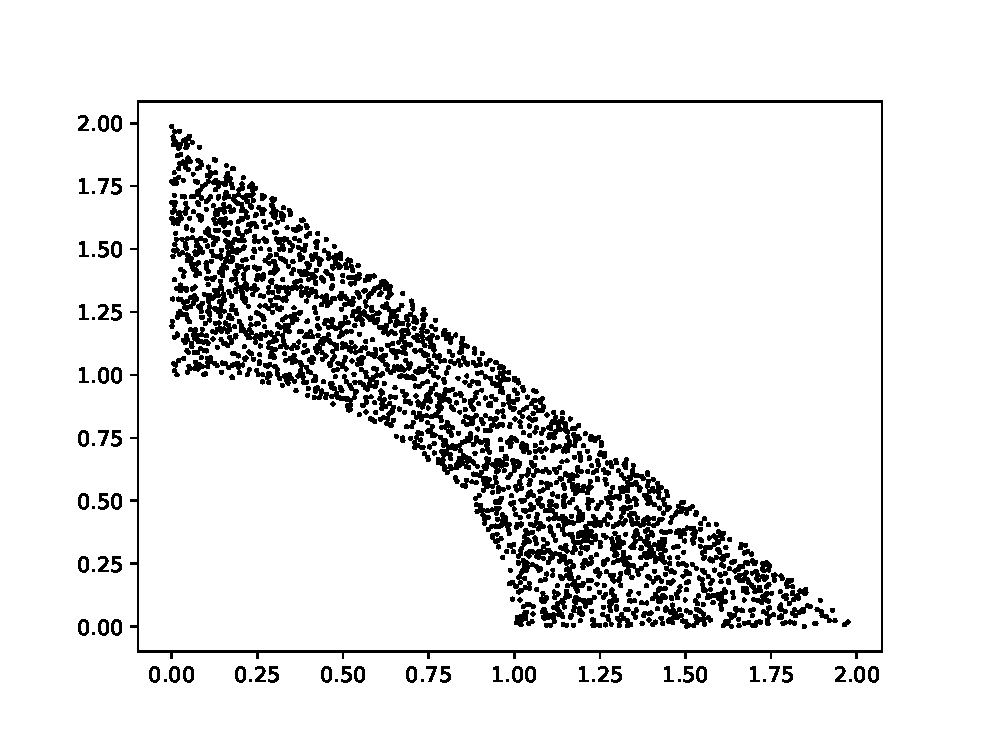
\includegraphics[width=0.9\textwidth]{rejection.eps}
%\centering
%\caption{Σημεία εκτέλεσης \textlatin{Monte Carlo}}
%\label{fig:rejection}
%\end{figure} 
%
%
%Παρακάτω ακολουθεί ο κώδικας που γράφτηκε σε \textlatin{Python} και έγινε χρήση της βιβλιοθήκης \textlatin{Numpy}.
%
%\selectlanguage{english}
%\lstinputlisting[style=python, firstline=8]{mc_rejection.py}

\end{document}